% !TeX program = xelatex
% !TeX encoding = UTF-8
\documentclass[UTF8]{standalone}
\usepackage{amsmath,newtxmath,esint,ctex,tikz}
\begin{document}
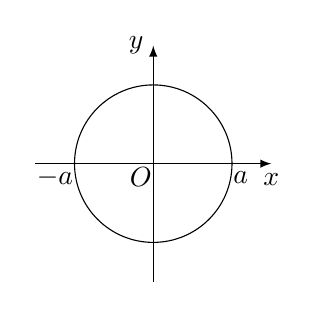
\begin{tikzpicture}
	\draw[domain=-3.14:3.14,smooth]
	plot[parametric,id=parametric-example,samples=100] function{cos(t)*cos(t)*cos(t),sin(t)*sin(t)*sin(t)};
	\draw[-latex] (-1.5,0) -- ++ (3,0) node[below] {$x$};
	\draw[-latex] (0,-1.5) -- ++ (0,3) node[left] {$y$};
	\draw (0,0) circle (1);
	\node[below=5pt,right=-3pt] at (1,0) {$a$};
	\node[below=5pt,left=-3pt] at (-1,0) {$-a$};
	\node[below=5pt,left=-3pt] at (0,0) {$O$};
\end{tikzpicture}
\end{document}